\documentclass{standalone}
\usepackage{tikz} % tikz
\usepackage{standalone} % tikz figures are often in standalone
\usepackage{amsfonts} % mathbb etc
\usepackage{amsmath} % crucial package
\usepackage{amsthm} % ams-style theorems
\usepackage{bm} % bold math symbols
\usepackage{xcolor} % more colors
\usepackage[T1]{fontenc} % modern encoding, better than OT1, the default

\newtheorem{definition-fr}{Définition}
\newtheorem{example-fr}{Exemple}
\newtheorem{theorem-fr}{Théorème}
\newtheorem{proposition-fr}{Proposition}
\newtheorem{lemma-fr}{Lemme}
\newtheorem{remark-fr}{Remarque}
\newtheorem{definition}{Definition}
\newtheorem{lemma}{Lemma}
\newtheorem{proposition}{Proposition}
\newtheorem{remark}{Remark}

\usetikzlibrary{decorations.pathmorphing} % for snake, zigzag...
\usetikzlibrary{positioning} % for the "below of=1cm" type of options
\usetikzlibrary{intersections} % e.g. for pyramid
\usetikzlibrary{calc} % for computing node coordinates from others
\usetikzlibrary{overlay-beamer-styles} % when \pause glitches in tikz beamer
\usetikzlibrary{arrows} % arrows
\usetikzlibrary{external} % only compile the figure the first time
\tikzexternalize[only named=true, prefix=tikz-cache/]
\immediate\write18{mkdir -p latex-build/tikz-cache}

% used to pass "scale=XX" as includetikz option
\pgfkeys{
  /tikzoptions/.is family, % Namespace
  /tikzoptions/.cd, % Namespace
  scale/.store in=\scale, % Store the value of 'scale'
}

% usage: \includetikz[scale=XX]{fig}, fetches from my local database
\newcommand{\includetikz}[2][scale=1]{
  \bgroup
  \pgfkeys{/tikzoptions,#1} % currently only accepts 'scale' (april 9 2025)
  \tikzsetnextfilename{#2}
  \include{tex-macros/tikz-figures/#2}% Include the standalone TikZ file
  \egroup
}

% usage: \inputtikz[scale=XX]{fig}, fetches from my local database
\newcommand{\inputtikz}[2][scale=1]{
  \bgroup
  \pgfkeys{/tikzoptions,#1} % currently only accepts 'scale' (april 9 2025)
  \tikzsetnextfilename{#2}
  \input{tex-macros/tikz-figures/#2}% Include the standalone TikZ file
  \egroup
}


\newcommand{\bigOt}{\widetilde{\mathcal{O}}}
\newcommand{\bigO}{\mathcal{O}}

\definecolor{mypurp}{HTML}{8f0c97}
\definecolor{myred}{HTML}{9f103b}
\definecolor{myor}{HTML}{ae3011}
\definecolor{mydarkor1}{HTML}{96240f}
\definecolor{mydarkor2}{HTML}{7f180c}
\definecolor{mylb1}{HTML}{00557e}
\definecolor{mylb2}{HTML}{013157}
\definecolor{mybl1}{HTML}{0d08a9}
\definecolor{mybl2}{HTML}{04037f}
\definecolor{mygr1}{HTML}{097e3e}
\definecolor{mygr2}{HTML}{025520}
\definecolor{myyellow}{HTML}{FFD700}



\makeatletter
\@ifundefined{scale}{
  \def\scale{1}
}
\makeatother


\begin{document}
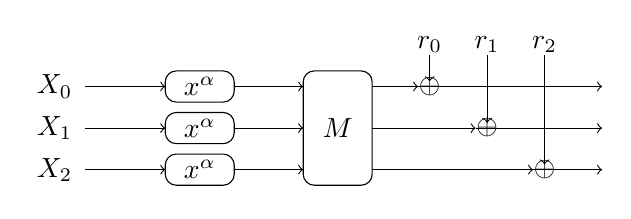
\begin{tikzpicture}[scale=\scale]
  \begin{scope}[xshift=0cm,xscale=0.146,yscale=0.066]
    \draw[->]   (0,0) node [left=1pt] {$X_0$} -- +(7,0);
    \draw[->]  (0,-8) node [left=1pt] {$X_1$} -- +(7,0);
    \draw[->]  (0,-16) node [left=1pt] {$X_2$} -- +(7,0);

    \draw[rounded corners]  (7,-3) rectangle node{$x^\alpha$} +(6,6);
    \draw[rounded corners]  (7,-11) rectangle node{$x^\alpha$} +(6,6);
    \draw[rounded corners]  (7,-19) rectangle node{$x^\alpha$} +(6,6);

    \draw[->]  (13,0) -- +(6,0);
    \draw[->]  (13,-8) -- +(6,0);
    \draw[->]  (13,-16) -- +(6,0);

    \draw[rounded corners]  (19,-19) rectangle node{$M$} +(6,22);

    \draw[->]  (25,0) -- +(4,0);
    \draw[->]  (29,0) -- +(16,0);

    \draw[->]  (25,-8) -- +(9,0);
    \draw[->]  (34,-8) -- +(11,0);

    \draw[->]  (25,-16) -- +(14,0);
    \draw[->]  (39,-16) -- +(6,0);

    \draw[->]  (30,8) node{$r_{0}$} ++(0,-2) -- +(0,-5);
    \draw[->]  (35,8) node{$r_{1}$} ++(0,-2) -- +(0,-13);
    \draw[->]  (40,8) node{$r_{2}$} ++(0,-2) -- +(0,-21);

    \draw  (30,0) node{$\oplus$} ;
    \draw  (35,-8) node{$\oplus$} ;
    \draw  (40,-16) node{$\oplus$} ;
  \end{scope}
\end{tikzpicture}
\end{document}
